\iffalse
\bibliography{../bib/thesis.bib}
\fi

\chapter{基于图的恶意软件静态分析方法研究}
\section{研究背景}

\section{基于图的恶意软件静态分析}
本方法的体系框架如图\ref{fig:chap1:Architecture}所示,由几个阶段构成。首先,反编译原始PE文件得到标准的汇编代码,经过预处理后抽象出控制流图(Control flow graph, CFG)。控制流图是用在编译器中的一个抽象数据结构,它是一个有向图,是过程或程序的抽象表现。在图中的每个节点代表一个基本块;每条有向边被用于代表在控制流中的跳跃,跳跃目标以一个块开始,以另一个块结束。其次,用调用的API或函数标记图中的每一条边,得到FA-CFG图;下一步,根据FA-CFG图建立特征向量,运用数据挖掘分类算法做出决策,判断该PE文件是否为恶意软件。

\begin{figure}[!ht]
\centering
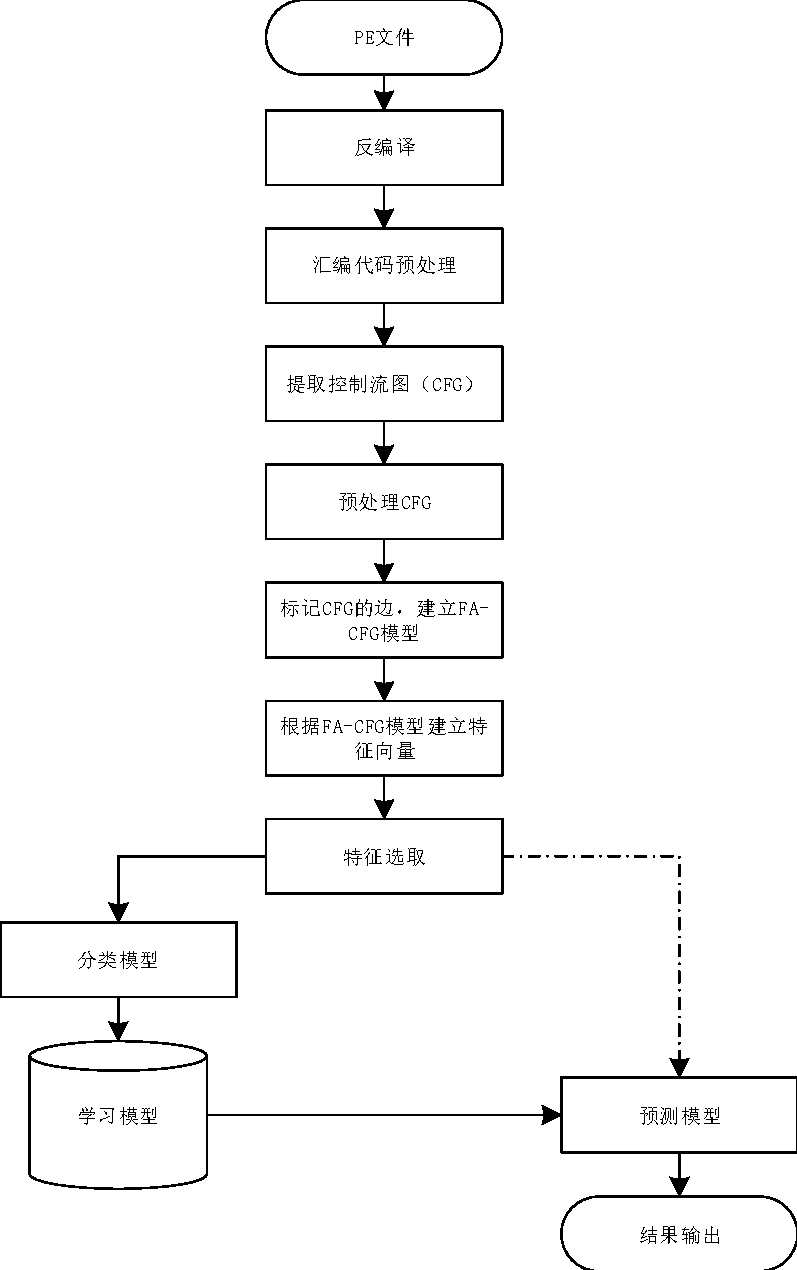
\includegraphics[width=4.5in]{img/chap1/Architecture.pdf}
\caption{体系框架图}
\label{fig:chap1:Architecture}
\end{figure}

如图\ref{fig:chap1:Architecture}所示,该方法由以下四个主要部分构成:PE文件反编译,FA-CFG图生成,特征提取、分类学习算法。第一步,通过反编译,得到输入PE文件的汇编代码;第二步,对得到的汇编代码进行预处理,移除一些不需要的指令代码,根据剩下的指令代码生成CFG图。根据API类库以及统计得到的调用函数的信息生成FA-CFG图。图中的一些边被对应的API或者调用函数的信息所标记。第三步,根据FA-CFG图提取特征,并采取主成分分析法(PCA)进行降维从而得到合理的特征向量。第四步,运用数据挖掘算法进行训练,形成学习模型。决策模块根据此模型判别一个输入PE文件是否为恶意。
\subsection{PE文件反编译及构建FA-CFG图}
静态分析方法中最主要的步骤是逆向工程。在静态分析中,通过检测代码来抓取恶意软件的行为。在不执行可疑软件的基础上使用逆向工程软件或反编译器来进行分析。逆向工程是编译的反过程,是从程序中以源代码的形式获得高层次的工程性描述或者说明的过程。它可以被用来对程序的执行计划、程序结构、算法进行仔细分析。在逆向工程的过程中,底层机器代码被反编译为汇编代码,进而汇编代码被反汇编成高级语言。通过逆向工程的分析可以得到程序的函数长度、可打印字符串、基本块、指令集、控制流图、调用关系图等信息。
在控制流图(CFG)中,每个节点代表一个基本块;每条有向边被用于代表在控制流中的跳跃,跳跃目标以一个块开始,以另一个块结束。在传统的控制流图中,每条边仅标识每次跳跃的开始与结束,没有反应跳跃的详细信息,包括调用的函数或API的信息等,因此,我们将函数调用和API调用产生的跳跃边用调用的详细进行标记,即可得到FA-CFG图。其中,函数调用所产生的边用所对应的函数的长度频率值标记,API调用所产生的边用对应API的ID标记。
\subsection{函数长度频率}
函数长度频率指函数代码长度在不同长度区间内的数量。将函数长度规模划分为几个不同的间隔,每个间隔称为一个容器。为每一个例子计算所有函数的长度在不同容器中的数量。由于函数长度的数量级差异,我们以指数增长的方式增加容器涵盖的范围。统计函数长度在1到$e$字节的数量,$e$字节到$e^{2}$字节的数量,以此类推。
